\documentclass[12pt]{article}
\usepackage{parskip}
\usepackage{amsmath}
\usepackage{pdfpages}
\usepackage{listings}
\usepackage{color}
\usepackage[margin=.6in]{geometry}

\definecolor{dkgreen}{rgb}{0,0.6,0}
\definecolor{gray}{rgb}{0.5,0.5,0.5}
\definecolor{mauve}{rgb}{0.58,0,0.82}

\lstset{frame=tb,
  language=C++,
  aboveskip=3mm,
  belowskip=3mm,
  showstringspaces=false,
  columns=flexible,
  basicstyle={\small\ttfamily},
  numbers=none,
  numberstyle=\tiny\color{gray},
  keywordstyle=\color{blue},
  commentstyle=\color{dkgreen},
  stringstyle=\color{mauve},
  breaklines=true,
  breakatwhitespace=true,
  tabsize=3
}



\begin{document}
\includepdf[pages=2]{slides.pdf}  
\includepdf[pages=3]{slides.pdf}  
You can send out a packet with all 1s for source ip and mac (called DHCP discover) to get a respose from the lan telling you each dchp server's mac address. DHCP sits inside UDP. We then can send a request to this thing whose mac address we know and they will respond with an available ip address. From this we can know that an ipaddress is available and bind to it. Then, for some reason an ARP request is sent to the dhcp server we were talking to just now. We advertise our ip and mac addresses as a bind. Basically the ARP request is you checking that it is ok to attempt to bind that ip address to your mac address (checking for conflicts). 

\includepdf[pages=4]{slides.pdf}  
\includepdf[pages=5]{slides.pdf}  
When a client attempts to bind to an ip they need to contact the server a bunch. The client sends out a discover packet telling the server what it needs. The server then responds with what the server has that might match those needs. From these options the client picks on and sends a request for that exact resource. The server then responds with an acknowledgement (could be positive or negative). The client then checks for conflicts using ARP and lets the server know the results (if we have bound to that or not).

This entire exchange, all packets have the same transaction id. The ARP exchanges are done to check that no one is configured with the selected IP address. We can shortcut this process because each offer is associeated with a lease time, renewal time, and rebinding time (lease time is greatest, renewal is least). When we already have an IP we just need to renew it which is much shorter. 

Each packet has something called a magic cookie. This is used to determine what kind of UDP packet it is (look into stun packets if you are curious).

\includepdf[pages=6]{slides.pdf}  
The idea is simple the application sucks. You have your local network that is not visible to the outside world. Packets with 10.0/8 should be reserved for local addresses (there should be no public addresses with this prefix). When you transition between local and public ipaddresses you have to multiplex. This is because many local ips will correspond to the same public ipaddress. The reverse is very hard since we only have one public ip address that has to route to multiple local addresses. 

\includepdf[pages=7]{slides.pdf}  
We want to have as many public ip addresses as sessions we want to have open to the internet. This way you have a public facing ip address that you can map each local address onto. 

\includepdf[pages=8]{slides.pdf}  
\includepdf[pages=9]{slides.pdf}  
\includepdf[pages=10]{slides.pdf}  
\includepdf[pages=11]{slides.pdf}  
Basically we try to use addresses from multiple layers to assist in multiplexing. We'll talk about tcp later.

Say we receive a packet that we have never seen before. We create an internal mapping from the public address to internal address. This mapping is maintained in memory only for the life time of the session. The session is essentially initialized when the internal host sends the first packet. From there a timer starts which allows us to assume that the session will be alive for 2 minutes (its super imprecise and can be configured). This is essentially a hole punched in your NAT device where we have assigned something and dont need to check. Everytime you see this kind of packet (same addresses and ports) it refreshes the session.

We want to retain the port number chosen by the internal host. Basically any mapping between addresses will be the port number for the public address. If two hosts chose the same internal port shit breaks, which is why we do conflict checking.

\includepdf[pages=12]{slides.pdf}  
For every device on the network you need to maintain a timer. When the internal host sends a packet corresponding to that session it should be refreshed. There is debate about whether this should happen when the external host sends a packet corresponding to the session. It could be a security flaw to do so, but not doing it might break applications with chatty external hosts and quite internal hosts.

\includepdf[pages=13]{slides.pdf}  
IP fragmentation fucks things up. Fragments might be missing the udp header which means that we don't have the ip addresses required for routing. We could make the NAT reassemble fragments but this is annoying and inefficient to do. What we ended up doing is that we don't allow them to exist at the same time. 

\includepdf[pages=14]{slides.pdf}  
\includepdf[pages=15]{slides.pdf}
Translation behavior = how you rewrite the packet  filetering behavior = how you determine which packets are allowed through

Endpoint independent behavior - For each thing you will have one mapping on the NAT device regardless of who the endpoint is. All packets destined for a address and port is allowed through if that device exists. This makes attacking easy because it doesn't even have to spoof its source ip address.

Address dependent behavior - There is a mapping for each thing, but things can share a mapping if they have the same endpoint ip (combine on ip address).

Address and port dependent behavior - There is a unique mapping for each endpoint value (combine on ip adress and port).


\includepdf[pages=16]{slides.pdf}
\textbf{Pairing} - when an internal host has several connections should be associated all of them with the same IP, we think yes

We run into problems when we need to preserve ports (conflicts and such).

Similarly port parity causes problems when people come up with crazy port mapping schemes that are hard to maintain.

\includepdf[pages=17]{slides.pdf}
When you're running a server behind a NAT device and something contacts it on a public port it should see public port of the device it connects to. Basically if you address me using my public port you should show me your public port. This is called hairpinning.

\includepdf[pages=18]{slides.pdf}
There is a protocol called TURN that helps with running a server behind NAT.








\end{document}